%\documentclass[compress]{beamer}
\documentclass[8pt]{beamer}

%-----------------------------------------------------------
% PACKAGES

%\usepackage[latin1]{inputenc}
\mode<presentation>

%\usepackage[T1]{fontenc}  
%\usetheme{Warsaw}
\usetheme{Frankfurt}

\usepackage{graphicx}
%\usepackage[section]{placeins} % force � mettre l'image o� on veut
%\usepackage{float} %utiliser H pour forcer � mettre l'image o� on veut
\usepackage{lscape} %utilisation du mode paysage
%\usepackage{pslatex}
\usepackage{url}
\usepackage{subfigure}

\usepackage{graphicx}
\usepackage{tabls}
\usepackage{afterpage}

%\usepackage[]{media9}
\usepackage{multimedia}

\usepackage{amsthm}
\usepackage{amssymb}
\usepackage{amsmath}
\usepackage{amsfonts}
\usepackage{amstext}
\usepackage{amsbsy}
\usepackage{mathbbol} 
\usepackage{mathrsfs}

\usepackage{epsfig}
%\usepackage{epsfig}
%\usepackage{cites}
\usepackage{epsf}
\usepackage{array}
\usepackage{color}
\usepackage{pdfpages}
\usepackage{cancel}

\usepackage{tikz}

\usepackage{multimedia}
\usepackage[]{media9}
%-----------------------------------------------------------
% NEW  DEFINITIONS
%
%=================================================================================================
% new commands
% +++++++++++++++++++++++++++++++++++++++++++++++++++++++++++++++++++++++++++++++++++++++++++++++++
\newcommand{\nc}{\newcommand}
%
% Ways of grouping things
%
\newcommand{\bracket}[1]{\left[ #1 \right]}
\newcommand{\bracet}[1]{\left\{ #1 \right\}}
\newcommand{\fn}[1]{\left( #1 \right)}
\newcommand{\ave}[1]{\left\langle #1 \right\rangle}
%
% Derivative forms
% 
\newcommand{\dx}[1]{\,d#1}
\newcommand{\dxdy}[2]{\frac{\partial #1}{\partial #2}}
\newcommand{\dxdt}[1]{\frac{\partial #1}{\partial t}}
\newcommand{\dxdz}[1]{\frac{\partial #1}{\partial z}}
\newcommand{\dfdt}[1]{\frac{\partial}{\partial t} \fn{#1}}
\newcommand{\dfdz}[1]{\frac{\partial}{\partial z} \fn{#1}}
\newcommand{\ddt}[1]{\frac{\partial}{\partial t} #1}
\newcommand{\ddz}[1]{\frac{\partial}{\partial z} #1}
\newcommand{\dd}[2]{\frac{\partial}{\partial #1} #2}
\newcommand{\ddx}[1]{\frac{\partial}{\partial x} #1}
\newcommand{\ddy}[1]{\frac{\partial}{\partial y} #1}
%
% Vector forms
%
%\renewcommand{\vec}[1]{\ensuremath{\stackrel{\rightarrow}{#1}}}
%\renewcommand{\div}{\ensuremath{\vec{\nabla} \cdot}}
%\newcommand{\grad}{\ensuremath{\vec{\nabla}}}

\renewcommand{\div}{\vec{\nabla}\! \cdot \!}
\newcommand{\grad}{\vec{\nabla}}
\newcommand{\oa}[1]{\fn{\frac{1}{3}\hat{\Omega}\!\cdot\!\overrightarrow{A_{#1}}}}

%
% Equation beginnings and endings
%
\newcommand{\bea}{\begin{eqnarray}}
\newcommand{\eea}{\end{eqnarray}}
\newcommand{\be}{\begin{equation}}
\newcommand{\ee}{\end{equation}}
\newcommand{\beas}{\begin{eqnarray*}}
\newcommand{\eeas}{\end{eqnarray*}}
\newcommand{\bdm}{\begin{displaymath}}
\newcommand{\edm}{\end{displaymath}}
%
% Equation punctuation
% 
\newcommand{\pec}{\hspace{0.25in},}
\newcommand{\pep}{\hspace{0.25in}.}
\newcommand{\pev}{\hspace{0.25in}}
%
% Equation labels and references, figure references, table references
% 
\newcommand{\LEQ}[1]{\label{eq:#1}}
\newcommand{\EQ}[1]{Eq.~(\ref{eq:#1})}
\newcommand{\EQS}[1]{Eqs.~(\ref{eq:#1})}
\newcommand{\REQ}[1]{\ref{eq:#1}}
\newcommand{\LFI}[1]{\label{fi:#1}}
\newcommand{\FI}[1]{Fig.~\ref{fi:#1}}
\newcommand{\RFI}[1]{\ref{fi:#1}}
\newcommand{\LTA}[1]{\label{ta:#1}}
\newcommand{\TA}[1]{Table~\ref{ta:#1}}
\newcommand{\RTA}[1]{\ref{ta:#1}}

%
% List beginnings and endings
% 
\newcommand{\bl}{\bss\begin{itemize}}
\newcommand{\el}{\vspace{-.5\baselineskip}\end{itemize}\ess}
\newcommand{\benu}{\bss\begin{enumerate}}
\newcommand{\eenu}{\vspace{-.5\baselineskip}\end{enumerate}\ess}
%
% Figure and table beginnings and endings
% 
\newcommand{\bfg}{\begin{figure}}
\newcommand{\efg}{\end{figure}}
\newcommand{\bt}{\begin{table}}
\newcommand{\et}{\end{table}}
%
% Tabular and center beginnings and endings
% 
\newcommand{\bc}{\begin{center}}
\newcommand{\ec}{\end{center}}
\newcommand{\btb}{\begin{center}\begin{tabular}}
\newcommand{\etb}{\end{tabular}\end{center}}
%
% Single space command
% 
%\newcommand{\bss}{\begin{singlespace}}
%\newcommand{\ess}{\end{singlespace}}
\newcommand{\bss}{\singlespacing}
\newcommand{\ess}{\doublespacing}
%
%---New environment "arbspace". (modeled after singlespace environment
%                                in Doublespace.sty)
%   The baselinestretch only takes effect at a size change, so do one.
% 
\def\arbspace#1{\def\baselinestretch{#1}\@normalsize}
\def\endarbspace{}
\newcommand{\bas}{\begin{arbspace}}
\newcommand{\eas}{\end{arbspace}}
%
% An explanation for a function
%
\newcommand{\explain}[1]{\mbox{\hspace{2em} #1}}
%
% Quick commands for symbols
%  
\newcommand{\half}{\frac{1}{2}}
\newcommand{\third}{\frac{1}{3}}
\newcommand{\twothird}{\frac{2}{3}}
\newcommand{\fourth}{\frac{1}{4}}
\newcommand{\mdot}{\dot{m}}
\newcommand{\ten}[1]{\times 10^{#1}\,}
\newcommand{\cL}{{\cal L}}
\newcommand{\cD}{{\cal D}}
\newcommand{\cF}{{\cal F}}
\newcommand{\cE}{{\cal E}}
\renewcommand{\Re}{\mbox{Re}}
\newcommand{\Ma}{\mbox{Ma}}
%
% Inclusion of Graphics Data
%
%\input{psfig}
%\psfiginit
%
% More Quick Commands
% 
\newcommand{\bi}{\begin{itemize}}
\newcommand{\ei}{\end{itemize}}
\newcommand{\ben}{\begin{enumerate}}
\newcommand{\een}{\end{enumerate}}
\newcommand{\dxi}{\Delta x_i}
\newcommand{\dyj}{\Delta y_j}
\newcommand{\ts}[1]{\textstyle #1}


\newcommand{\bu}{\boldsymbol{u}}
\newcommand{\ber}{\boldsymbol{e}}
\newcommand{\br}{\boldsymbol{r}} 
\newcommand{\bo}{\boldsymbol{\Omega}}

\newcommand{\bn}{\boldsymbol{\nabla}}

% DGFEM commands
\newcommand{\jmp}[1]{[\![#1]\!]}                     % jump
\newcommand{\mvl}[1]{\{\!\!\{#1\}\!\!\}}             % mean value


\newcommand{\boxedeqn}[1]{%
  \[\fbox{%
      \addtolength{\linewidth}{-2\fboxsep}%
      \addtolength{\linewidth}{-2\fboxrule}%
      \begin{minipage}{\linewidth}%
      \begin{equation}#1\end{equation}%
      \end{minipage}%
    }\]%
}
\newcommand{\mboxed}[1]{\boxed{\phantom{#1}}}
\newcommand{\ud}{\,\mathrm{d}}

% keff
\newcommand{\keff}{\ensuremath{k_{\textit{eff}}}}

% margin par
\newcommand{\mt}[1]{\marginpar{ {\footnotesize #1} }}

% shortcut for aposterio in italics
\newcommand{\apost}{\textit{a posteriori\xspace}}
\newcommand{\Apost}{\textit{A posteriori}\xspace}

% shortcut for multi-group
\newcommand{\mg}{multigroup\xspace}
\newcommand{\Mg}{Multigroup\xspace}
\newcommand{\ho}{higher-order\xspace}
\newcommand{\Ho}{Higher-order\xspace}
\newcommand{\HO}{Higher-Order\xspace}
\newcommand{\HObig}{HIGHER-ORDER\xspace}
\newcommand{\Mgbig}{MULTIGROUP\xspace}

% shortcut for domain notation
\newcommand{\D}{\mathcal{D}}

% shortcut for xuthus
\newcommand{\psc}[1]{{\sc {#1}}}
\newcommand{\xuthus}{\psc{xuthus}\xspace}

% vector shortcuts
\newcommand{\vo}{\vec{\Omega}}
\newcommand{\vr}{\vec{r}}
\newcommand{\vn}{\vec{n}}
\newcommand{\vnk}{\vec{\mathbf{n}}}

% extra space
\newcommand{\qq}{\quad\quad}

% sign function
\DeclareMathOperator{\sgn}{sgn}


\newcommand{\ensuretext}[1]{\ensuremath{\text{#1}}}

% common reference commands
\newcommand{\eqt}[1]{Eq.~(\ref{#1})}                     % equation
\newcommand{\fig}[1]{Fig.~\ref{#1}}                      % figure
\newcommand{\tbl}[1]{Table~\ref{#1}}                     % table



\newcommand{\rhs}{right-hand-side\xspace}
\newcommand{\clearemptydoublepage}{\newpage{\pagestyle{empty}\cleardoublepage}}


\newcommand{\bs}[1]{\mathbf{#1}}
\renewcommand{\bs}[1]{\vec{#1}}
%\newcommand{\dd}{\mathrm{d}}
\newcommand{\norm}{\textrm{norm}}
\renewcommand{\Re}{\textrm{Re}}
\newcommand{\Pe}{\textrm{P\'e}}
\renewcommand{\Pr}{\textrm{Pr}}

\newcommand{\resi}{R_e}
%\newcommand{\resinew}{\tilde{D}_e}
\newcommand{\resinew}{\widetilde{\resi}}
\newcommand{\matder}[1]{\frac{\textrm{D} #1}{\textrm{D} t}}

\newcommand{\divv}[1]{\vec{\nabla}^{#1}\! \cdot \!}
\newcommand{\gradd}[1]{\vec{\nabla}^{#1}}

\newcommand{\tcr}[1]{\textcolor{red}{#1}}
\newcommand{\tcb}[1]{\textcolor{blue}{#1}}
\newcommand{\tcm}[1]{\textcolor{magenta}{#1}}

\renewcommand{\L}{\mathbf{L}}
\renewcommand{\S}{\mathbf{\Sigma}}
\newcommand{\M}{\mathbf{M}}
\renewcommand{\D}{\mathbf{D}}
%=================================================================================================

%============================================================

%style et couleur
%\usetheme{Frankfurt}
\date{\today}

%\addtobeamertemplate{footline}{\hfill\insertframenumber/\inserttotalframenumber\hspace{2em}\null}

\setbeamertemplate{footline}{
\leavevmode%
%\hbox{\hspace*{-0.06cm}
\begin{beamercolorbox}[wd=.5\paperwidth,ht=3.25ex,dp=1ex,center]{author in head/foot}%
	\usebeamerfont{author in head/foot}\insertshortauthor%~~(\insertshortinstitute)
\end{beamercolorbox}%
\begin{beamercolorbox}[wd=.25\paperwidth,ht=3.25ex,dp=1ex,center]{section in head/foot}%
	\usebeamerfont{section in head/foot} IQS NEAMS 2015 % \insertshorttitle
\end{beamercolorbox}%
\begin{beamercolorbox}[wd=.25\paperwidth,ht=3.25ex,dp=1ex,left]{section in head/foot}%
	\usebeamerfont{section in head/foot}\insertshortdate{}\hspace*{2em}
	\insertframenumber{} / \inserttotalframenumber %\hspace*{2ex}
\end{beamercolorbox}}%
%\vskip0pt%
%}

\beamertemplatetransparentcovered

\urldef{\ragusa}\url{jean.ragusa@tamu.edu}

\title{TREAT Mission Supporting Problem\\
Improved Quasi-Static Method in RattleSnake}

\author{Jean C. Ragusa, Zach M. Prince}
\institute{Department of Nuclear Engineering, Texas A\&M University, College Station, TX}

%%%%%%%%%%%%%%%%%%%%%%%%%%%%%%%%%%%%%%%%%%%%%%%%%%%%%%%%%%%%%%%%%%%%

%%%%%%%%%%%%%%%%%%%%%%%%%%%%%%%%%%%%%%%%%%%%%%%%%%%%%%%%%%%%%%%%%%%%
%%%%%%%%%%%%%%%%%%%%%%%%%%%%%%%%%%%%%%%%%%%%%%%%%%%%%%%%%%%%%%%%%%%%
\begin{document}
%%%%%%%%%%%%%%%%%%%%%%%%%%%%%%%%%%%%%%%%%%%%%%%%%%%%%%%%%%%%%%%%%%%%
%%%%%%%%%%%%%%%%%%%%%%%%%%%%%%%%%%%%%%%%%%%%%%%%%%%%%%%%%%%%%%%%%%%%

%-------------------------------------------------------------------
\begin{frame}
%\vspace{-1.5cm}
	\begin{figure}[t]
		\centering
			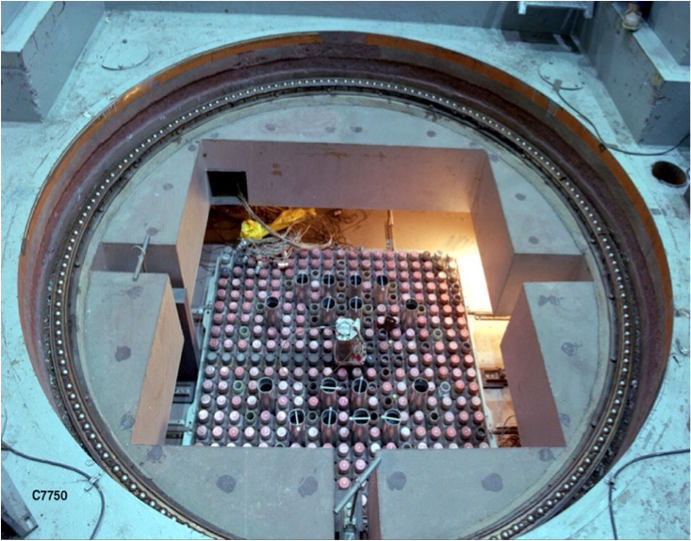
\includegraphics[width=.45\textwidth]{figures/Treat_core_view.png}
	\end{figure}
\vspace{-0.5cm}
\titlepage
\small{email: {\ragusa} }

\end{frame}
%-------------------------------------------------------------------

%-------------------------------------------------------------------
\begin{frame}
	\frametitle{Outline}
	\tableofcontents 
\end{frame}
%-------------------------------------------------------------------

%%%%%%%%%%%%%%%%%%%%%%%%%%%%%%%%%%%%%%%%%%%%%%%%%%%%%%%%%%%%%%%%%%%%
%%%%%%%%%%%%%%%%%%%%%%%%%%%%%%%%%%%%%%%%%%%%%%%%%%%%%%%%%%%%%%%%%%%%
\section{Theory}
%%%%%%%%%%%%%%%%%%%%%%%%%%%%%%%%%%%%%%%%%%%%%%%%%%%%%%%%%%%%%%%%%%%%
%%%%%%%%%%%%%%%%%%%%%%%%%%%%%%%%%%%%%%%%%%%%%%%%%%%%%%%%%%%%%%%%%%%%

%%%%%%%%%%%%%%%%%%%%%%%%%%%%%%%%%%%%%%%%%%%%%%%%%%%%%%%%%%%%%%%%%%%%
\subsection{Time-dependent Multigroup Transport}
%%%%%%%%%%%%%%%%%%%%%%%%%%%%%%%%%%%%%%%%%%%%%%%%%%%%%%%%%%%%%%%%%%%%

%-------------------------------------------------------------------
\begin{frame}{Time-dependent Multigroup Transport}


\begin{block}{Fluxes $(1 \le g \le G )$}
\begin{multline}
\frac{1}{v^g}\frac{\partial \Psi^g ( \vec{r},\vec{\Omega },t) }{\partial t} 
=
\sum_{g^\prime=1}^{G} \int\nolimits_{4\pi }d\Omega ^{\prime }
\left[
\Sigma _{s}^{g^\prime\to g}(\vec{r},\vec{\Omega ^{\prime }} \cdot \vec{\Omega },t)
+ 
\frac{\chi _{p}^g}{4\pi } \nu_{p}\Sigma ^{g^\prime}_{f}(\vec{r},t)
\right]
\Psi^{g^\prime} ( \vec{r},\vec{\Omega ^{\prime }},t)  \\
% 
-div\left[ \vec{\Omega }\Psi ^g ( \vec{r},\vec{\Omega },t) \right]
-\Sigma ^g(\vec{r},t)\Psi ^g( \vec{r},\vec{\Omega },t) 
%
+\sum\limits_{i=1}^{I} \frac{\chi ^g _{d,i}(\vec{r})}{4\pi} \lambda _{i}C_{i}(\vec{r},t)  \notag 
\end{multline}
+ IC + BC \\
\medskip
In operator notation:
\begin{equation*}
\boxed{
\frac{1}{v}\frac{\partial \Psi }{\partial t} = (H + P_p - L) \Psi  + S_{d} 
}
\end{equation*}
\end{block}

\vspace{-4mm}

\begin{block}{Precursors $C_i$ $(1 \le i \le I)$}
\begin{equation*}
\boxed{
\frac{dC_i}{dt} = \sum_{g=1}^G \nu_{d,i}^{g} \Sigma_f^g(\vec{r},t) \Phi^{g}(\vec{r},t) - \lambda_i(\vec{r},t) C_i(\vec{r},t) 
}
\end{equation*}
%with
%\be
%\beta = \sum_{i=1}^I \beta_{i} 
%\ee
\end{block}

\end{frame}
%-------------------------------------------------------------------
%
%%%%%%%%%%%%%%%%%%%%%%%%%%%%%%%%%%%%%%%%%%%%%%%%%%%%%%%%%%%%%%%%%%%%%
%\subsection{Time-dependent Multigroup Diffusion}
%%%%%%%%%%%%%%%%%%%%%%%%%%%%%%%%%%%%%%%%%%%%%%%%%%%%%%%%%%%%%%%%%%%%%
%
%%-------------------------------------------------------------------
%\begin{frame}{Time-dependent Multigroup Diffusion}
%
%
%\begin{block}{Equations}
%Neutron flux $\phi^g$:
%\begin{align}
%\frac{1}{v^g} \frac{\partial \phi^g }{\partial t} =& \frac{\chi_p^g}{\keff} \sum_{g'=1}^G (1-\beta) \nu^{g'} \Sigma_f^{g'} \phi^{g'} -  \left( -\div D^g \grad  + \Sigma_r^g \right) \phi^g  \nonumber \\
%&  + \sum_{g'\neq g}^G\Sigma_s^{g'\to g} \phi^{g'}  + \sum_{i=1}^I\chi_{d,i}^g\lambda_i C_i \ , \quad 1 \le g \le G 
%\end{align}
%Precursors $C_i$
%\be
%\frac{dC_i}{dt} = \frac{\beta_i}{k_{eff}}\sum_{g=1}^G\nu^{g} \Sigma_f^g \phi^{g} - \lambda_i C_i \ , \quad 1 \le i \le I 
%\ee
%with
%\be
%\beta = \sum_{i=1}^I \beta_{i} 
%\ee
%\end{block}
%
%\end{frame}
%%-------------------------------------------------------------------

%%%%%%%%%%%%%%%%%%%%%%%%%%%%%%%%%%%%%%%%%%%%%%%%%%%%%%%%%%%%%%%%%%%%
\subsection{Factorization approach}
%%%%%%%%%%%%%%%%%%%%%%%%%%%%%%%%%%%%%%%%%%%%%%%%%%%%%%%%%%%%%%%%%%%%

%-------------------------------------------------------------------
\begin{frame}{Flux Factorization}

\begin{block}{Factorization}
Decomposition of the multigroup flux into the \tcm{product} of a time-dependent \tcr{amplitude} ($p$) and a space-/time-dependent multigroup \tcb{shape} ($\psi$):
\begin{equation*}
\boxed{
\Psi^g(\vec{r},\vec{\Omega},t) = \tcr{p(t)} \tcb{\psi^g (\vec{r},\vec{\Omega},t)}
}
\end{equation*}
and, for the scalar flux,
\begin{equation*}
\boxed{
\Phi^g(\vec{r},t) = \tcr{p(t)} \tcb{\varphi^g(\vec{r},t)}
}
\end{equation*}
with, obviously,
\begin{equation*}
\varphi^g(\vec{r},t) = \int_{4\pi} d\Omega^\prime\, \psi^g(\vec{r},\vec{\Omega}^\prime,t)
\end{equation*}
\end{block}

\begin{block}{}
\begin{itemize}
\item 
Factorization is \tcm{not} an approximation
\item
When reporting these in the previous equations, one obtains to the so-called \tcb{shape} equations.
\item
Note that \tcm{factorization is not unique}: 
\[
\Psi= \tcr{p} \times \tcb{\psi} = \tcr{\frac{p}{a}} \times \tcb{\left( a \psi \right)}
\]
\end{itemize}
\end{block}

\end{frame}
%-------------------------------------------------------------------

%%%%%%%%%%%%%%%%%%%%%%%%%%%%%%%%%%%%%%%%%%%%%%%%%%%%%%%%%%%%%%%%%%%%
\subsection{IQS equations}
%%%%%%%%%%%%%%%%%%%%%%%%%%%%%%%%%%%%%%%%%%%%%%%%%%%%%%%%%%%%%%%%%%%%

%-------------------------------------------------------------------
\begin{frame}{Shape equations}

\begin{block}{Shape equations}
The shape equations are similar to the original transport equations:
\begin{equation*}
\boxed{
\frac{1}{v}\frac{\partial \tcb{\psi} }{\partial t} = (H + P_p - \tcb{\tilde{L}}) \tcb{\psi}  + \tcr{\frac{1}{p}} S_{d} 
}
\end{equation*}
%\begin{align}
%\frac{1}{v^g} \frac{\partial \varphi^g }{\partial t} =& \frac{\chi_p^g}{\keff} \sum_{g'=1}^G (1-\beta) \nu^{g'} \Sigma_f^{g'} \varphi^{g'} -  \left( -\div D^g \grad  + \Sigma_r^g + \tcr{\frac{1}{v^g}\frac{1}{p}\frac{dp}{dt}}\right) \varphi^g  \nonumber \\
%&  + \sum_{g'\neq g}^G\Sigma_s^{g'\to g} \varphi^{g'}  + \tcr{\frac{1}{p}}\sum_{i=1}^I\chi_{d,i}^g\lambda_i C_i \ , \quad 1 \le g \le G 
%\label{eq:shape}
%\end{align}
\begin{equation*}
\boxed{
\frac{dC_i}{dt} = \sum_{g=1}^G \nu_{d,i}^{g} \Sigma_f^g(\vec{r},t) \tcr{p} \tcb{\varphi^{g}}(\vec{r},t) - \lambda_i(\vec{r},t) C_i(\vec{r},t) 
}
\end{equation*}
%\be
%\frac{dC_i}{dt} = \frac{\beta_i}{k_{eff}}\sum_{g=1}^G\nu^{g} \Sigma_f^g \tcr{p} \varphi^{g} - \lambda_i C_i \ , \quad 1 \le i \le I 
%\ee
\end{block}

\begin{block}{Differences with original transport equation}
\ben
\item An additional removal term based on $\tcr{\frac{1}{v^g}\frac{1}{p}\frac{dp}{dt}} \tcb{\psi^g}$
\vspace{-3mm}
\begin{equation*}
\boxed{
\tcb{\tilde{L}^g} = L^g + \tcr{\frac{1}{v^g}\frac{1}{p}\frac{dp}{dt}} 
}
\end{equation*}
\vspace{-3mm}
\item Delayed neutron source term scaled by $\tcr{\frac{1}{p}}$
\item \tcm{No change} in the precursor equations but we have re-written them to show explicitly  $\tcr{p} \times \tcb{\varphi^{g}}$
\een
\end{block}

\end{frame}
%-------------------------------------------------------------------

%-------------------------------------------------------------------
\begin{frame}{Shape equations: Implementation within the MOOSE framework}

\begin{block}{Shape equations $\to$ \tcr{FEM solver + implicit time integration}}
\begin{equation*}
\boxed{
\frac{1}{v}\frac{\tcb{\psi}^{n+1}-\tcb{\psi}^n }{\Delta t} = \left(H^{n+1} + P_p^{n+1} - L^{n+1} -\tcr{\frac{1}{v}\frac{1}{p^{n+1}}\left.\frac{dp}{dt}\right|_{n+1}} \right) \tcb{\psi}^{n+1}  + \tcr{\frac{1}{p^{n+1}}} S_{d}^{n+1} 
}
\end{equation*}
\end{block}

\begin{block}{Modification to the original transport equation}
\ben
\item An additional removal term based on $\tcr{\frac{1}{v^g}\frac{1}{p}\frac{dp}{dt}} \tcb{\psi^g}$\\
\tcm{$\to$ add a new kernel}
\item Delayed neutron source term scaled by $\tcr{\frac{1}{p}}$\\
\tcm{$\to$ scale the delayed neutron source kernel}
\item nonlinear coupling between shape variable $\tcb{\psi^{n+1}}$ and amplitude variable $\tcr{p^{n+1}}$
\een
\end{block}

\end{frame}
%-------------------------------------------------------------------

%%%%%%%%%%%%%%%%%%%%%%%%%%%%%%%%%%%%%%%%%%%%%%%%%%%%%%%%%%%%%%%%%%%%
% \subsection{Amplitude equations}
%%%%%%%%%%%%%%%%%%%%%%%%%%%%%%%%%%%%%%%%%%%%%%%%%%%%%%%%%%%%%%%%%%%%

%-------------------------------------------------------------------
\begin{frame}{Amplitude equations (PRKE)}

\begin{block}{Principle}
To obtain the \tcr{amplitude} equation, we multiply the shape equations with a weighting 
function (initial adjoint flux, $\Psi^*$), then integrate over phase-space.  
\end{block}

\begin{block}{Notation}
For brevity, the adjoint flux product and integration over phase-space will be represented with parenthetical notation:
\[
\int_{4\pi}\int_D\Psi^{*g}(\vec{r},\vec{\Omega})f^g(\vec{r},\vec{\Omega})d^3rd\Omega=\left(\Psi^{*g},f^g\right)
\]
\end{block}


\begin{block}{Uniqueness of the factorization}
In order to impose uniqueness of the factorization, one requires:
\[
\tcr{K_0} = \sum_{g=1}^G\left(\Psi^{*g},\frac{1}{v^g}\psi^g\right)= constant
\]
\end{block}


\end{frame}
%-------------------------------------------------------------------

%-------------------------------------------------------------------
\begin{frame}{PRKE (continued)}

\begin{block}{PRKE}
\[
\frac{d\tcr{p}}{dt}=\left[\frac{\rho-\bar{\beta}}{\Lambda}\right]\tcr{p}+\sum_{i=1}^I\bar{\lambda}_i\xi_i
\]
\[
\frac{d\xi_i}{dt}=\frac{\bar{\beta}_i}{\Lambda}\tcr{p} - \bar{\lambda}_i\xi_i \quad 1 \le i \le I 
\]
\end{block}

\begin{block}{PRKE Coefficients}
\[
\frac{\rho-\bar{\beta}}{\Lambda}=
\frac{ \left( \Psi^{*}, (H+P_p-L) \tcb{\psi} \right)}{K_0}
\]
\[
\frac{\bar{\beta}}{\Lambda}=\sum_{i=1}^I\frac{\bar{\beta}_i}{\Lambda}=
\sum_{i=1}^I \frac{ \left(\Psi^{*}, P_{d,i} \tcb{\psi} \right)}{K_0}
\]
\[
\bar{\lambda}_i=\frac{(\Psi^{*},\chi_{d,i}\lambda_i \tcb{C_i})}{(\Psi^{*},\chi_{d,i}\tcb{C_i})}
\]
\end{block}

\end{frame}
%-------------------------------------------------------------------

%%%%%%%%%%%%%%%%%%%%%%%%%%%%%%%%%%%%%%%%%%%%%%%%%%%%%%%%%%%%%%%%%%%%
\subsection{IQS method solution process}
%%%%%%%%%%%%%%%%%%%%%%%%%%%%%%%%%%%%%%%%%%%%%%%%%%%%%%%%%%%%%%%%%%%%

%-------------------------------------------------------------------
\begin{frame}{Coupling}

\begin{block}{Factorization leads to a \tcr{nonlinear} system}
The amplitude and shape equations form a system of \tcr{nonlinear} coupled equations: 
\ben
\item the coefficients appearing in the \tcr{PRKE}s depend upon the \tcb{shape} solution,
\item the \tcb{shape} equation has a kernel dependent on \tcr{amplitude} and its derivative,  
\item the delayed neutron source term is scaled by the amplitude.
\een
\end{block}

\begin{block}{Time scales and IQS method solution process}
Because solving for the shape can be expensive, especially in two or three dimensions, it is attractive to make the assumption that the shape is weakly time-dependent so the shape can be computed after a multitude of PRKE calculations which is the root of IQS: 
%

\begin{figure}[h]
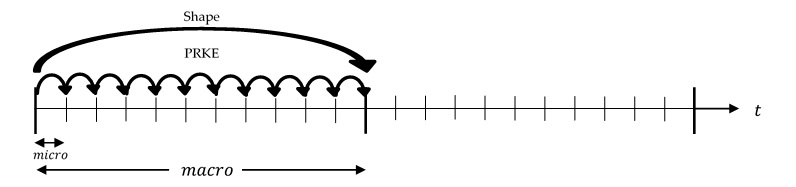
\includegraphics[width=\linewidth]{figures/IQS_visualization.jpg}
%\caption{IQS method solution process}
\label{fig:IQS}
\end{figure}

\end{block}
\end{frame}
%-------------------------------------------------------------------

%-------------------------------------------------------------------
\begin{frame}{Convergence criteria}


\begin{block}{Ideally}
The normalization constant should not change over time !
\[
\tcr{K_0} = \sum_{g=1}^G\left(\Psi^{*g},\frac{1}{v^g}\psi^g(\tcr{t=0})\right)= constant
\]
\[
\text{Thus, we employ }\quad
\left| \frac{\sum_{g=1}^G\left(\Psi^{*g},\frac{1}{v^g}\psi^g(\tcb{t=t^{n+1}})\right)}{\tcr{K_0}}-1\right| 
= \left| \frac{\tcb{K_{n+1}}}{{\tcr{K_0}}}-1\right|  < tol
\]
\end{block}

\begin{block}{Note that we have seen in practice ... }
\[
\frac{ \| \psi^{g,_{t_{n+1}}^{\tcr{\ell+1}}} - \psi^{g,_{t_{n+1}}^{\tcr{\ell}}} \|}{\| \psi^{g,_{t_{n+1}}^{\tcr{\ell+1}}} \|} < tol 
\quad \text{or even} \quad
\frac{ \| \psi^{g,_{t_{n+1}}^{\tcr{\ell+1}}} - \psi^{g,_{t_{n+1}}^{\tcr{0}}} \|}{\| \psi^{g,_{t_{n+1}}^{\tcr{0}}} \|} < tol 
\]
where $\tcr{\ell}=$IQS iteration index over a given macro time step $[t_n,t_{n+1}]$\\
\smallskip
These empirical criteria must be followed by a renormalization before starting the next time step $[t_{n+1},t_{n+2}]$
\[
\psi^{g,_{t_{n+1}}^{\tcr{converged}}} \leftarrow \psi^{g,_{t_{n+1}}^{\tcr{converged}}} \times \frac{K_{n+1}^{\tcr{converged}}}{K_0}
\]
\end{block}


\end{frame}
%-------------------------------------------------------------------

%%%%%%%%%%%%%%%%%%%%%%%%%%%%%%%%%%%%%%%%%%%%%%%%%%%%%%%%%%%%%%%%%%%%
\subsection{Precursors time-discretization}
%%%%%%%%%%%%%%%%%%%%%%%%%%%%%%%%%%%%%%%%%%%%%%%%%%%%%%%%%%%%%%%%%%%%

%-------------------------------------------------------------------
\begin{frame}{Precursors time-discretization}

A simple ODE:
\begin{equation*}
\boxed{
\frac{dC_i}{dt} = \sum_{g=1}^G \nu_{d,i}^{g} \Sigma_f^g(\vec{r},t) \tcr{p} \tcb{\varphi^{g}}(\vec{r},t) - \lambda_i(\vec{r},t) C_i(\vec{r},t) 
}
\end{equation*}
\begin{block}{Numerical integration: Theta-scheme (already in RattleSnake)}
\be
C^{n+1} = \frac{1-(1-\theta)\Delta t\lambda}{1+\theta\Delta t\lambda}C^n 
+ \frac{(1-\theta)\Delta t \beta (\nu\Sigma_f)^n}    {1+\theta\Delta t\lambda}\tcb{\varphi^n}     \tcr{p^n }
+ \frac{\theta\Delta t     \beta (\nu\Sigma_f)^{n+1}}{1+\theta\Delta t\lambda}\tcb{\varphi^{n+1}} \tcr{p^{n+1}}
\ee
Reporting this value of $C^{n+1}$ in $S_d^{n+1}$, one can solve for the shape $\psi^{n+1}$ as a function of $\psi^n$ and $C^n$
(and $p^n$, $p^{n+1}$, $dp/dt|_n$ and  $dp/dt|_{n+1}$).\\

\bigskip
Once $\psi^{n+1}$ has been determined, $C^{n+1}$ is updated. \\

\medskip
RattleSnake currently implements both implicit ($\theta=1$) and Crank-Nicholson ($\theta=1/2$) as options for precursor evaluation.

\end{block}

\end{frame}
%-------------------------------------------------------------------

%-------------------------------------------------------------------
\begin{frame}{Analytical Integration}


\begin{block}{Analytical Integration}
\[
C^{n+1} =  C^n e^{-\lambda (t_{n+1} - t_n) }  + \int_{t_n}^{t_{n+1}} \nu_d\Sigma_f(t')\tcb{\varphi(t')} \tcr{p(t')} e^{-\lambda (t_{n+1}-t')}dt'
\]
\end{block}

\begin{block}{}
Assuming a \tcm{linear in time variation} over the macro time step $[t_n, t_{n+1}]$ for the \tcb{shape} and the \tcb{fission cross section}, we get:
\[
C^{n+1} = C^n e^{-\lambda \Delta t} 
+ \left[\tcm{a_3}(\nu_d\Sigma_f)^{n+1}+\tcm{a_2}(\nu_d\Sigma_f)^n\right]\tcb{\varphi^{n+1}}
+ \left[\tcm{a_2}(\nu_d\Sigma_f)^{n+1}+\tcm{a_1}(\nu_d\Sigma_f)^n\right]\tcb{\varphi^n    }
\]
where the integration coefficients are defined as:
\begin{align}
&a_1 = \int_{t_n}^{t_{n+1}}\left(\frac{t_{n+1}-t'}{\Delta t}\right)^2 \tcr{p(t')} e^{-\lambda(t_{n+1}-t')}dt' \notag \\
&a_2= \int_{t_n}^{t_{n+1}}\frac{(t'-t_n)(t_{n+1}-t')}{(\Delta t)^2}   \tcr{p(t')} e^{-\lambda(t_{n+1}-t')}dt'   \notag \\
&a_3 = \int_{t_n}^{t_{n+1}}\left(\frac{t'-t_n}{\Delta t}\right)^2     \tcr{p(t')} e^{-\lambda(t_{n+1}-t')}dt'     \notag 
\end{align}


The amplitude $\tcr{p}$ is contained in the $a_i$'s integration coefficients.\\
\tcr{$p(t)$} has been \tcm{accurately} calculated at the \tcm{micro time} step level.

\end{block}

\end{frame}
%-------------------------------------------------------------------

%%-------------------------------------------------------------------
%\begin{frame}{Analytical Integration (continued)}
%
%Recall that we just need to compute  coefficients of the form:
%\[
%\int_{t_n}^{t_{n+1}}\left(\delta_2 t'^2 + \delta_1 t' +\delta_0\right) \tcr{p(t')}e^{-\lambda(t_{n+1}-t')}dt' 
%\]
%
%\begin{block}{}
%
%The amplitude $(p)$ is contained in the $a_i$'s integration coefficients.\\
%$p(t)$ has been highly accurately calculated at the micro time step level.
%
%\end{block}
%
%\end{frame}
%%-------------------------------------------------------------------

%%%%%%%%%%%%%%%%%%%%%%%%%%%%%%%%%%%%%%%%%%%%%%%%%%%%%%%%%%%%%%%%%%%%
%%%%%%%%%%%%%%%%%%%%%%%%%%%%%%%%%%%%%%%%%%%%%%%%%%%%%%%%%%%%%%%%%%%%
\section{Implementation in RATTLESNAKE}
%%%%%%%%%%%%%%%%%%%%%%%%%%%%%%%%%%%%%%%%%%%%%%%%%%%%%%%%%%%%%%%%%%%%
%%%%%%%%%%%%%%%%%%%%%%%%%%%%%%%%%%%%%%%%%%%%%%%%%%%%%%%%%%%%%%%%%%%%

\subsection{Changes to RATTLESNAKE}

%-------------------------------------------------------------------
\begin{frame}{Changes to RATTLESNAKE}

\begin{block}{Action Systems}
\bi
\item Continuous FEM Diffusion (\tcr{completed})
\item Discontinuous FEM Diffusion
\item Discontinuous FEM Sn Transport (first-order form)
\item Discontinuous FEM Sn Transport (SAAF form)
\ei
Four action systems \tcr{$\ne$} four times the work!
\end{block}

\begin{block}{}
\bi
\item \tcm{Action System} (adding IQS as an option)
\item Post-processors (\tcm{element integrals}) for PRKE coefficients: $\rho-\bar{\beta}$, $\bar{\beta}_i$, $\bar{\lambda}_i$\\
Note that the numerator of $\rho-\bar{\beta}$, i.e., $\left( \Psi^{*}, (H+P_p-L) \psi \right)$, is particularly easy thanks to the residual {\tt save\_in} option of MOOSE.
\item IQS \tcm{userobject} (PRKE solve using updated PRKE coefficients)
\item IQS \tcm{executioner} derived from MOOSE executioner (use of the existing Picard iteration loop in the {\tt transient} executioner; this can seamlessly enable IQS in multiphysics simulations without any further changes)
\ei
\end{block}

\end{frame}
%-------------------------------------------------------------------


%-------------------------------------------------------------------
\begin{frame}{}


\begin{block}{Break down of IQS Changes}
\begin{figure}[h]
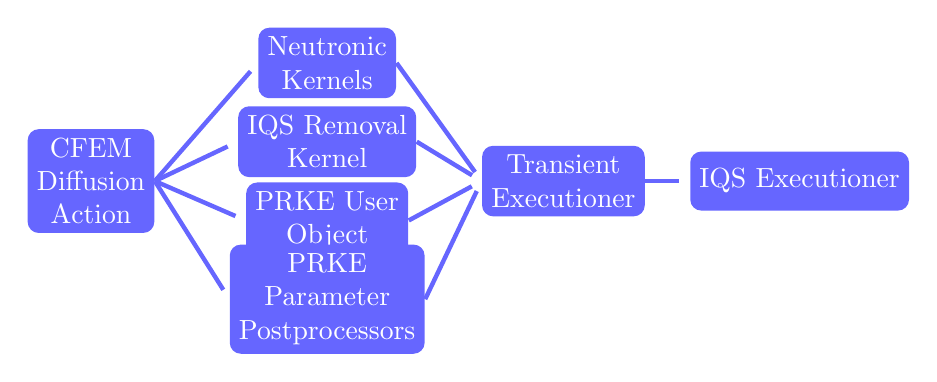
\begin{tikzpicture}[every node/.style = {shape          = rectangle, rounded corners, fill = blue!60, minimum width  = 1.5cm, minimum height = 0.75cm, align= center, text = white},blue edge/.style  = { -, ultra thick, blue!60, shorten >= 4pt}]
\node(0;0) at (-1,0) {CFEM \\ Diffusion \\ Action};
  \node(1;3)  at (2, 1.5) {Neutronic \\ Kernels};   
  \node(1;1)  at (2, 0.5) {IQS Removal \\ Kernel}; 
  \node(1;-1)  at (2,-0.5) {PRKE User \\ Object}; 
  \node(1;-3) at (2,-1.5) {PRKE \\ Parameter \\ Postprocessors}; 
     \node(2;0)  at (5,0) {Transient \\ Executioner};
     	\node(3;0)  at (8,0) {IQS Executioner};
\foreach \j in {-3,-1,1,3}
  { \draw[blue edge] (0;0.east) -- (1;\j.west); }
\foreach \j in {-3,-1,1,3}
  { \draw[blue edge] (1;\j.east) -- (2;0.west);} 
\draw[blue edge] (2;0.east) -- (3;0.west);         
\end{tikzpicture}
%\caption{CFEM Diffusion Action Process Diagram}   
\label{Action}
\end{figure}
\end{block}

\end{frame}
%-------------------------------------------------------------------

%%%%%%%%%%%%%%%%%%%%%%%%%%%%%%%%%%%%%%%%%%%%%%%%%%%%%%%%%%%%%%%%%%%%
%%%%%%%%%%%%%%%%%%%%%%%%%%%%%%%%%%%%%%%%%%%%%%%%%%%%%%%%%%%%%%%%%%%%
\section{Results}
%%%%%%%%%%%%%%%%%%%%%%%%%%%%%%%%%%%%%%%%%%%%%%%%%%%%%%%%%%%%%%%%%%%%
%%%%%%%%%%%%%%%%%%%%%%%%%%%%%%%%%%%%%%%%%%%%%%%%%%%%%%%%%%%%%%%%%%%%


%%%%%%%%%%%%%%%%%%%%%%%%%%%%%%%%%%%%%%%%%%%%%%%%%%%%%%%%%%%%%%%%%%%%
\subsection{TWIGL benchmark}
%%%%%%%%%%%%%%%%%%%%%%%%%%%%%%%%%%%%%%%%%%%%%%%%%%%%%%%%%%%%%%%%%%%%

%-------------------------------------------------------------------
\begin{frame}{TWIGL benchmark}

\begin{figure}[h]
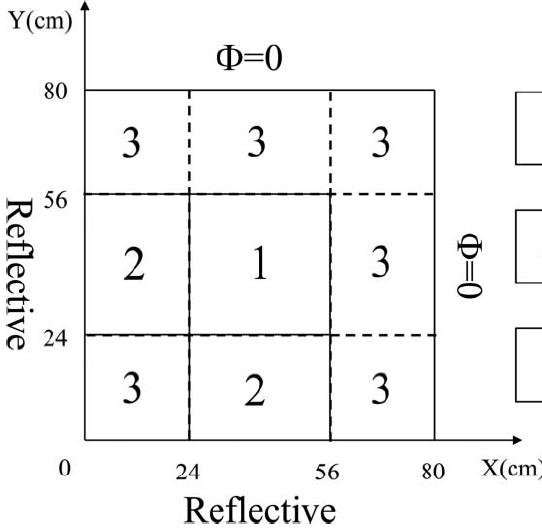
\includegraphics[width=\linewidth]{figures/twigl_geom.png}
%\caption{IQS method solution process}
\label{fig:IQS}
\end{figure}

\end{frame}
%-------------------------------------------------------------------

%-------------------------------------------------------------------
\begin{frame}{TWIGL:  Computational Efficacy}

Relative error versus \# of linear iterations:
\begin{figure}[h]
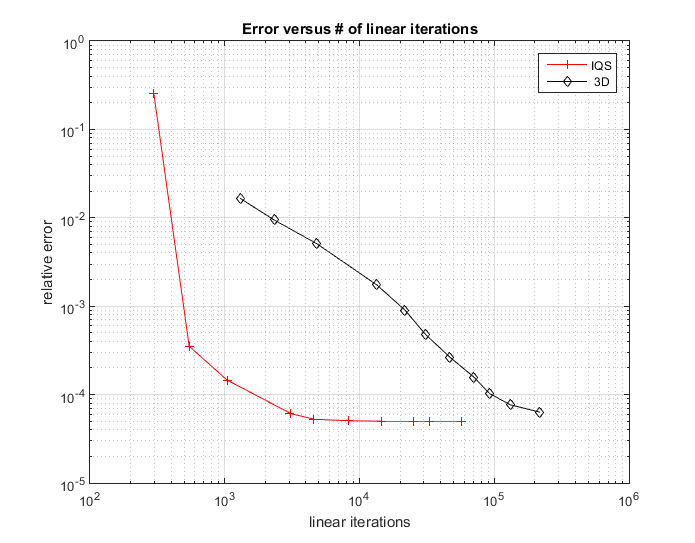
\includegraphics[width=0.9\linewidth]{figures/twigl_convergence_iqs.png}
%\caption{IQS method solution process}
\label{fig:IQS}
\end{figure}

\end{frame}
%-------------------------------------------------------------------

\begin{frame}{TWIGL:  Shape and flux movies (thermal group)}
%  \begin{columns}
%    \column{.5\textwidth}
%       \includemedia[addresource=ndiff_twigl_ramp_03.mpg, activate=pageopen, deactivate=pageclose, width=6.5cm, height=5cm, flashvars={source=ndiff_twigl_ramp_03.mpg & autoPlay=true & loop=true }]{}{VPlayer.swf}
%    \column{.5\textwidth}
%      \includemedia[addresource=iqs_twigl_ramp_03.mpg, activate=pageopen, deactivate=pageclose, width=6.5cm, height=5cm, flashvars={source=iqs_twigl_ramp_03.mpg & autoPlay=true & loop=true }]{}{VPlayer.swf}
%  \end{columns}
\begin{center}
\movie[width=5cm,height=4cm,showcontrols=true,externalviewer]{IQS}{iqs_twigl_ramp_03.mpg}
\movie[width=5cm,height=4cm,showcontrols=true,externalviewer]{Flux}{ndiff_twigl_ramp_03.mpg}
\end{center}
\end{frame}

%%%%%%%%%%%%%%%%%%%%%%%%%%%%%%%%%%%%%%%%%%%%%%%%%%%%%%%%%%%%%%%%%%%%%%%%%%%%%%%%%%%%%%%

%{
%\setbeamercolor{background canvas}{bg=}
%\includepdf[pages={9-24}]{./PDT-Scaling-MLA-DH-TS-TST-May14-final.pdf}
%\includepdf[pages={26}]{./PDT-Scaling-MLA-DH-TS-TST-May14-final.pdf}
%}

%%%%%%%%%%%%%%%%%%%%%%%%%%%%%%%%%%%%%%%%%%%%%%%%%%%%%%%%%%%%%%%%%%%%%

%{
%\setbeamercolor{background canvas}{bg=}
%\includepdf[pages={-}]{./RagusaPresentationV3-Copy.pdf}
%}

%%%%%%%%%%%%%%%%%%%%%%%%%%%%%%%%%%%%%%%%%%%%%%%%%%%%%%%%%%%%%%%%%%%%%

%%%%%%%%%%%%%%%%%%%%%%%%%%%%%%%%%%%%%%%%%%%%%%%%%%%%%%%%%%%%%%%%%%%%%
%%%%%%%%%%%%%%%%%%%%%%%%%%%%%%%%%%%%%%%%%%%%%%%%%%%%%%%%%%%%%%%%%%%%%
\section{Wrap-up}
%%%%%%%%%%%%%%%%%%%%%%%%%%%%%%%%%%%%%%%%%%%%%%%%%%%%%%%%%%%%%%%%%%%%%
%%%%%%%%%%%%%%%%%%%%%%%%%%%%%%%%%%%%%%%%%%%%%%%%%%%%%%%%%%%%%%%%%%%%%

%-------------------------------------------------------------------
\begin{frame}{Conclusion and Outlook}

\begin{block}{Completed}
\bi
\item Theoretical understanding of IQS convergence and selection of proper convergence criteria
\item 1D prototype Matlab code for MOOSE comparison/verification
\item IQS userobject and executioner (using Picard iterations)
\item IQS for \tcr{CFEM Diffusion} action system
\ei
\end{block}

\begin{block}{In progress}
\bi
\item Implementation of analytical precursor integration in YAK
\item Further YAK verification
\item YAK documentation
\ei
\end{block}
\begin{block}{Next Steps}
\bi
\item DFEM Diffusion action system
\item DFEM SN Transport action system
\item Kinetics benchmarks (neutronics only, e.g., TWIGL, LMW)
\item Dynamics benchmarks (with feedback, e.g., the LRA test case)
\item Study of a JFNK-based algorithm to resolve the IQS nonlinearity between the amplitude/shape equations
\ei
\end{block}

\end{frame}
%-------------------------------------------------------------------

%-------------------------------------------------------------------
\begin{frame}{Questions ?}


\begin{block}{Thanks}
\begin{itemize}
\item Yaqi Wang (INL, RattleSnake code lead)
\item Mark DeHart (INL, TREAT M\&S lead)
\item NEAMS
\end{itemize}

\begin{block}{}
\begin{figure}
	\centering
	\includegraphics[scale=0.3]{./crunching.png}
\end{figure}
\end{block}

\end{block}

\end{frame}
%-------------------------------------------------------------------


%%-------------------------------------------------------------------
%\begin{frame}{}
%
%
%\begin{block}{}
%\end{block}
%
%\end{frame}
%%-------------------------------------------------------------------

%%%%%%%%%%%%%%%%%%%%%%%%%%%%%%%%%%%%%%%%%%%%%%%%%%%%%%%%%%%%%%%%%%%%
%%%%%%%%%%%%%%%%%%%%%%%%%%%%%%%%%%%%%%%%%%%%%%%%%%%%%%%%%%%%%%%%%%%%
%\begin{frame}{Thank you}
%
%\begin{block}{Computational Transport}
%\begin{figure}
%	\centering
%	\includegraphics[scale=0.33]{./fig/crunching.png}
%\end{figure}
%\end{block}
%
%\end{frame}
%%%%%%%%%%%%%%%%%%%%%%%%%%%%%%%%%%%%%%%%%%%%%%%%%%%%%%%%%%%%%%%%%%%%
%%%%%%%%%%%%%%%%%%%%%%%%%%%%%%%%%%%%%%%%%%%%%%%%%%%%%%%%%%%%%%%%%%%%

%************************************************

\end{document}